% tikzpic.tex
\documentclass[crop,tikz]{standalone}% 'crop' is the default for v1.0, before it was 'preview'
%\usetikzlibrary{...}% tikz package already loaded by 'tikz' option

\usepackage{amsmath}
\usepackage{mathtools}
\usepackage{amssymb,amsthm}
\usepackage[normalem]{ulem}
\usepackage{bm}
\usepackage{pgfplots}

\usepackage{pgf}
\usepackage{tikz}
\usepackage[utf8]{inputenc}
\usetikzlibrary{arrows,automata}
\usetikzlibrary{positioning}
\usetikzlibrary{shapes,fit} %use shapes library if you need ellipse

\usepackage{tikz}
\usetikzlibrary{positioning,calc}

\usetikzlibrary{intersections}
\tikzset{
    state/.style={
           rectangle,
           rounded corners,
           draw=black, very thick,
           minimum height=2em,
           inner sep=2pt,
           text centered,
           },
    state2/.style={
           rectangle,
           rounded corners,
           draw=black,
           minimum height=2em,
           inner sep=2pt,
           text centered,
           },
}


\begin{document}

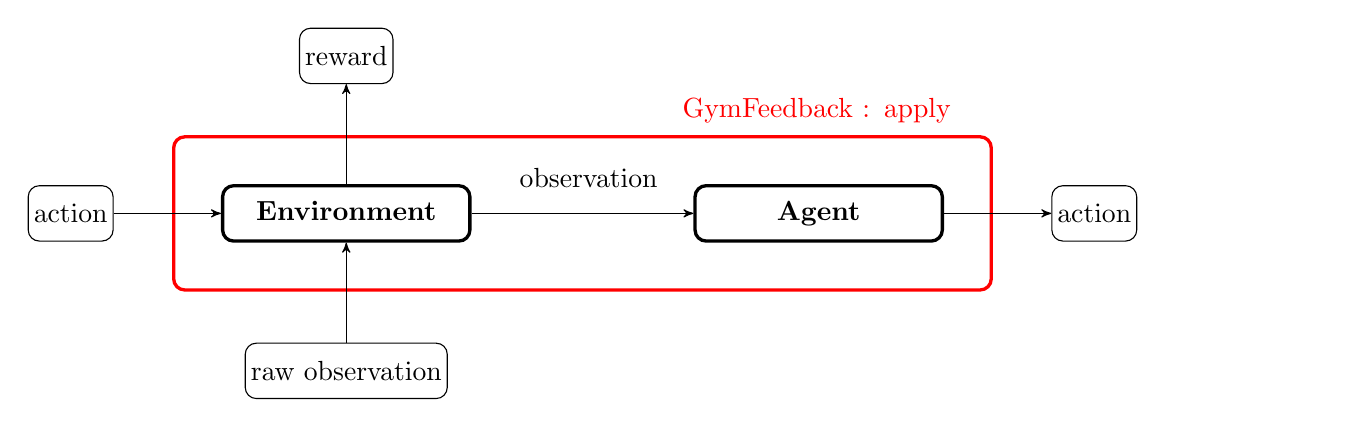
\begin{tikzpicture}
[
->,>=stealth'
]

 % First node
 % Use previously defined 'state' as layout (see above)
 % use tabular for content to get columns/rows
 % parbox to limit width of the listing


 \node[state2,
 node distance=5cm] (ACTIN) 
 {%
action
 };


 % Next node: RAKE
 \node[state,       % layout (defined above)
 node distance=3.5cm,     % distance to QUERY
 right of=ACTIN,
 text width=3cm,        % max text width
 %yshift=+3cm
 ] (ENV)    % move 3cm in y
  {%                     % posistion relative to the center of the 'box'
 \begin{tabular}{l}     % content
  \textbf{Environment}
 \end{tabular}
 };
 
 \node[state2,
 above of=ENV,
 node distance=2cm] (REWARD) 
 {%
reward
 };



 % STATE ACK
 \node[state,
 right of=ENV,
 node distance=6cm,
 text width=3cm] (AGENT) 
  {%                     % posistion relative to the center of the 'box'
 \begin{tabular}{l}     % content
  \textbf{Agent}\\
 \end{tabular}
 };


 % STATE EPC
 \node[state2,
 below of=ENV,
 node distance=2cm] (RAWOBS) 
 {%
raw observation
 };

 \node[state2,
 right of=AGENT,
 node distance=3.5cm] (ACTOUT) 
 {%
action
 };
 
 
\node[state,draw=red, fit=(ENV) (AGENT),inner sep=6mm](GYMFEEDBACK) {};
 
 % draw the paths and and print some Text below/above the graph
 \path 
 (GYMFEEDBACK)
  node[anchor=north,text width=8cm,yshift=4.5em, xshift=15em]{\color{red}GymFeedback : apply} 
  (GYMFEEDBACK)
 (ACTIN) edge (ENV)
 (ENV) edge   
  node[anchor=north,below,text width=3cm,yshift=2em, xshift=2em]{observation} 
  (AGENT)
  (RAWOBS) edge (ENV)
  (AGENT) edge (ACTOUT)
  (ENV) edge (REWARD)
 ;
\end{tikzpicture}

\end{document}